\documentclass[11pt]{article}

\newcommand{\cnum}{CS188}
\newcommand{\ced}{Winter 2017}
\newcommand{\ctitle}[3]{\title{\vspace{-0.5in}\cnum, \ced\\Problem Set #1: #2\\Due #3}}
\usepackage{enumitem}
\usepackage{amsmath}
\newcommand{\solution}[1]{{{\color{blue}{\bf Solution:} {#1}}}}
\usepackage[usenames,dvipsnames,svgnames,table,hyperref]{xcolor}
\usepackage{graphicx}
\renewcommand*{\theenumi}{\alph{enumi}}
\renewcommand*\labelenumi{(\theenumi)}
\renewcommand*{\theenumii}{\roman{enumii}}
\renewcommand*\labelenumii{\theenumii.}


\begin{document}
\ctitle{1}{Decision Trees}{Feb. 2,2017}
\author{}
\date{}
\maketitle
\vspace{-0.75in}

\section{Problem 1}
\begin{enumerate}
\item Problem 1a

\solution{
\[L(\theta) = P(X_1,X_2, ...X_n ; \theta) \]
Due to independence,
\[
L(\theta) = P(X_{1}; \theta) * P(X_{2}; \theta) * ... P(X_{n} ; \theta) = \prod_{i = 1}^{n} P(X_{i}; \theta)
\]
Since \[X_i  Ber(p): \]
\[P(X_i ; \theta) = \theta^{X_i}(1 - \theta)^{1 - X_i}, X_i \in [0,1] \]
Thus,
\[ L(\theta) = \prod_{i=1}^{n} \theta^{X_i}(1 - \theta)^{1 - X_i} \]
The likelihood does not depend on the order of the random variables, since they are independent. 
}

\vspace{1cm}
\item Problem 1b

\solution{
\[l(\theta) = log(L(\theta)) = log \prod_{i = 1}^{N} \theta^{X_i}(1 - \theta)^{1 - X_i} = \sum_{i = 1}^{N} log(\theta^{X_i}(1 - \theta)^{1 - X_i})\]

\[ l(\theta) = \sum_{i = 1}^{N}(X_{i}log(\theta) + (1 - X_{i})log(1 - \theta)) \]
\[ \frac{\delta l}{\delta \theta} = \sum_{i = 1}^{N}(\frac{X_i}{\theta} - \frac{1 - X_i}{1 - \theta}) \]
Setting \[ \sum_{i = 1}^{N} X_i = \bar{X} \]
\[ \frac{\delta l}{\delta \theta} = n(\frac{\bar{X}}{\theta} - \frac{1 - \bar{X}}{1 - \theta}) \]
\[ \frac{\delta^{2}l}{\delta \theta^{2}} = n(-\frac{\bar{X}}{\theta^{2}} - \frac{1 - \bar{X}}{(1 - \theta)^{2}}) \]
\[ \frac{\delta l}{\delta \theta} = 0 \longrightarrow{} \theta = \bar{X} = \sum_{i = 1}^{N} X_i \]
Since \[ \frac{\delta^2 l}{\delta \theta^2} < 0 \] at \[ \theta = \bar{X} \] \[ \theta = \bar{X} = \sum_{i = 1}^{N} X_i \] is the MLE.

}

\vspace{1cm}
\item Problem 1c
\solution{ \newline{}
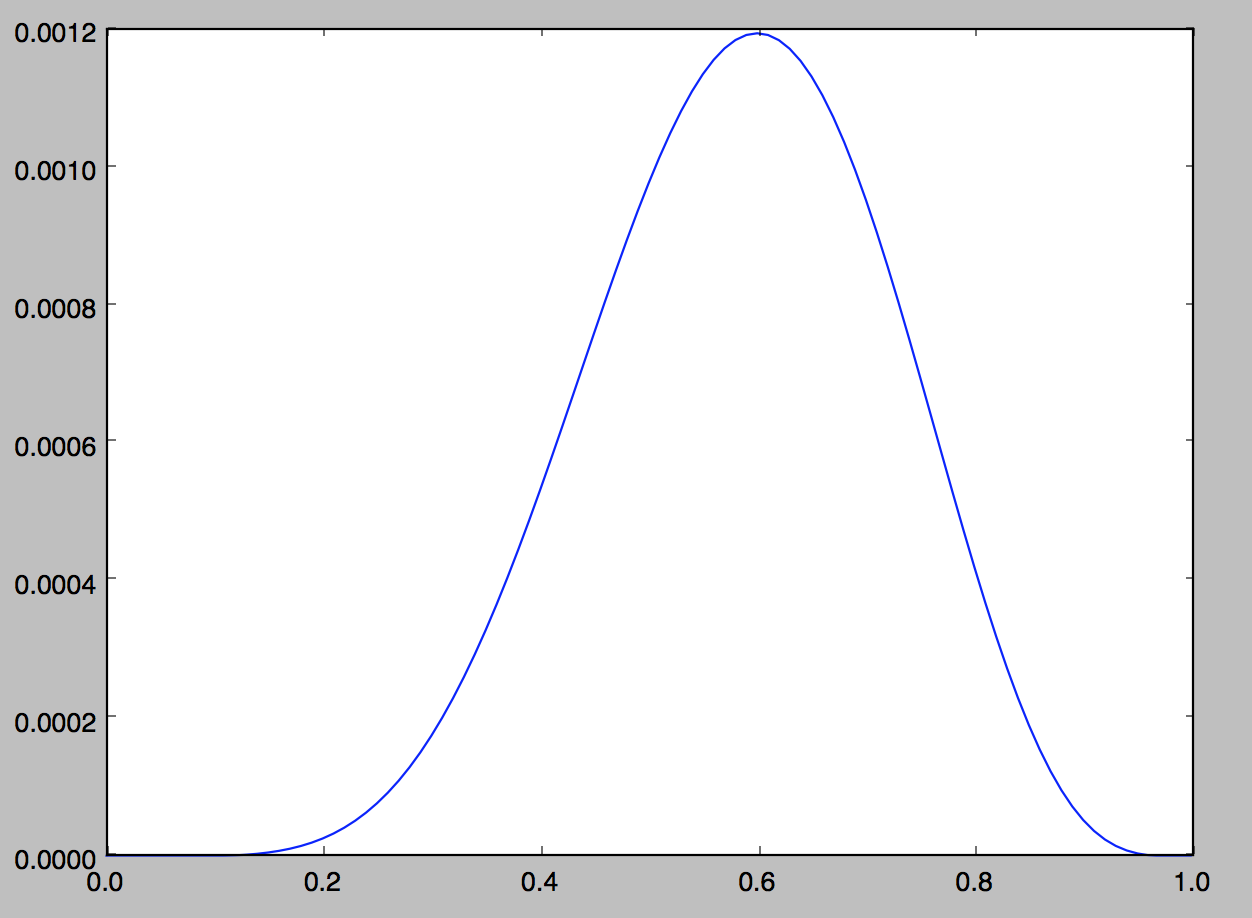
\includegraphics[scale=0.5]{1CPlot.png} \newline{}
The maximum can clearly be seen to occur at theta = 0.6 (the computer finds the max to occur at 0.599999...). This agrees with the closed form answer since from the data, we calculate that \[ \bar{X} = 0.6 \]
}

\item Problem 1d
\solution{
Plot for n = 5, three 1's:
\newline{}
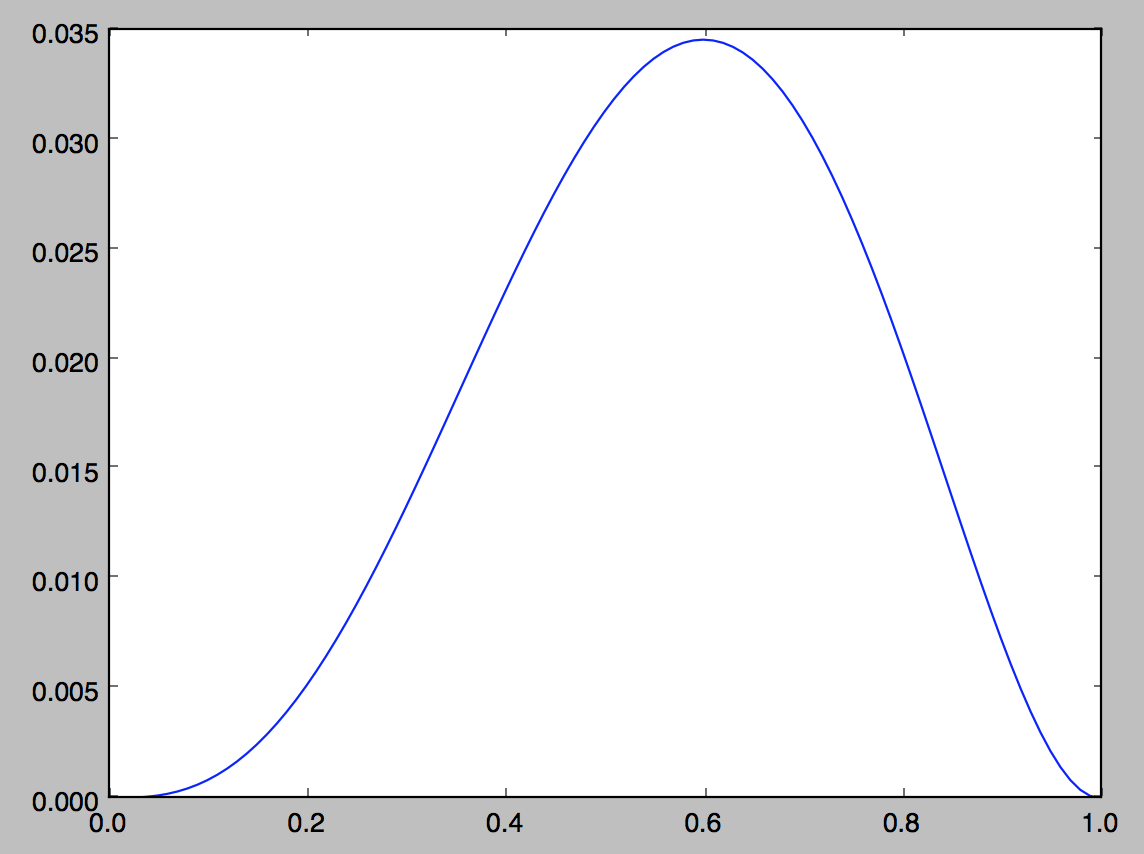
\includegraphics[scale=0.5]{threeones.png} \newline{}
Plot for n = 100, 60 ones: 
\newline{}
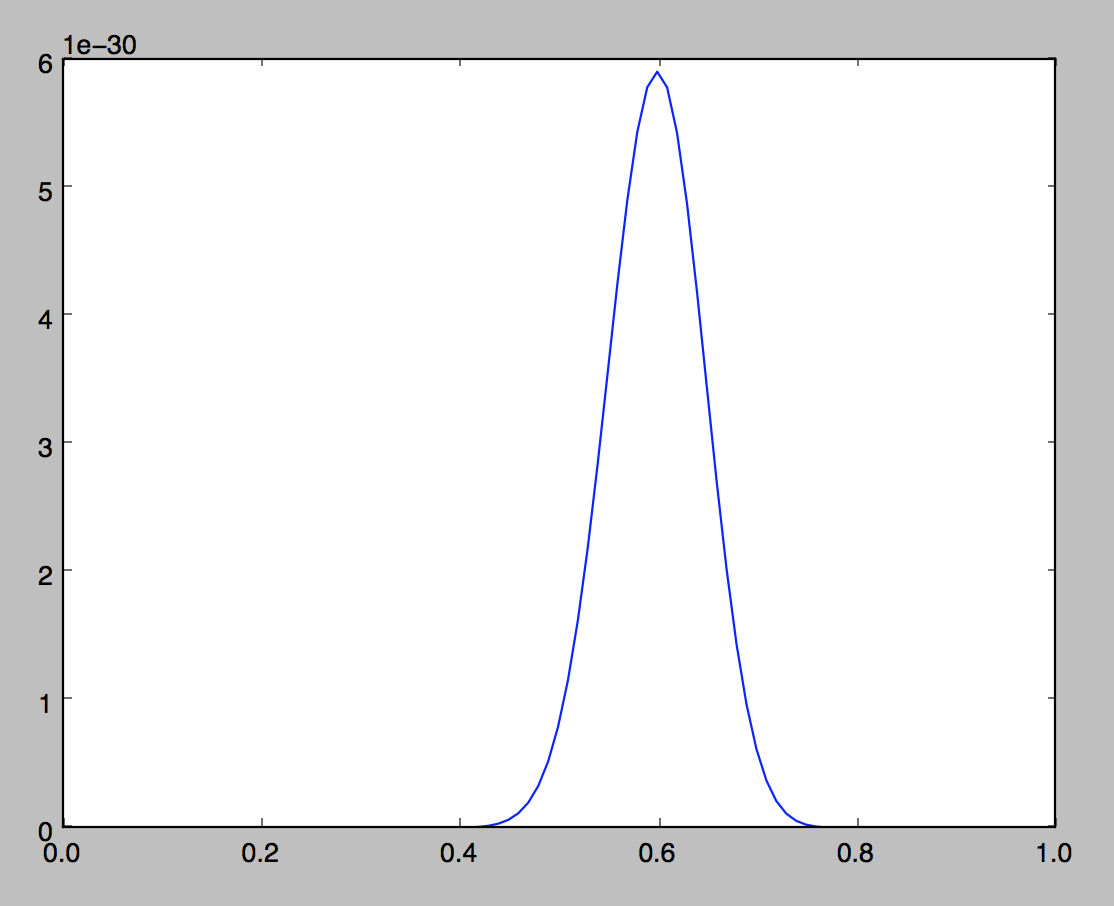
\includegraphics[scale=0.5]{sixtyones.png} \newline{}
Plot for n = 10, 5 ones: 
\newline{}
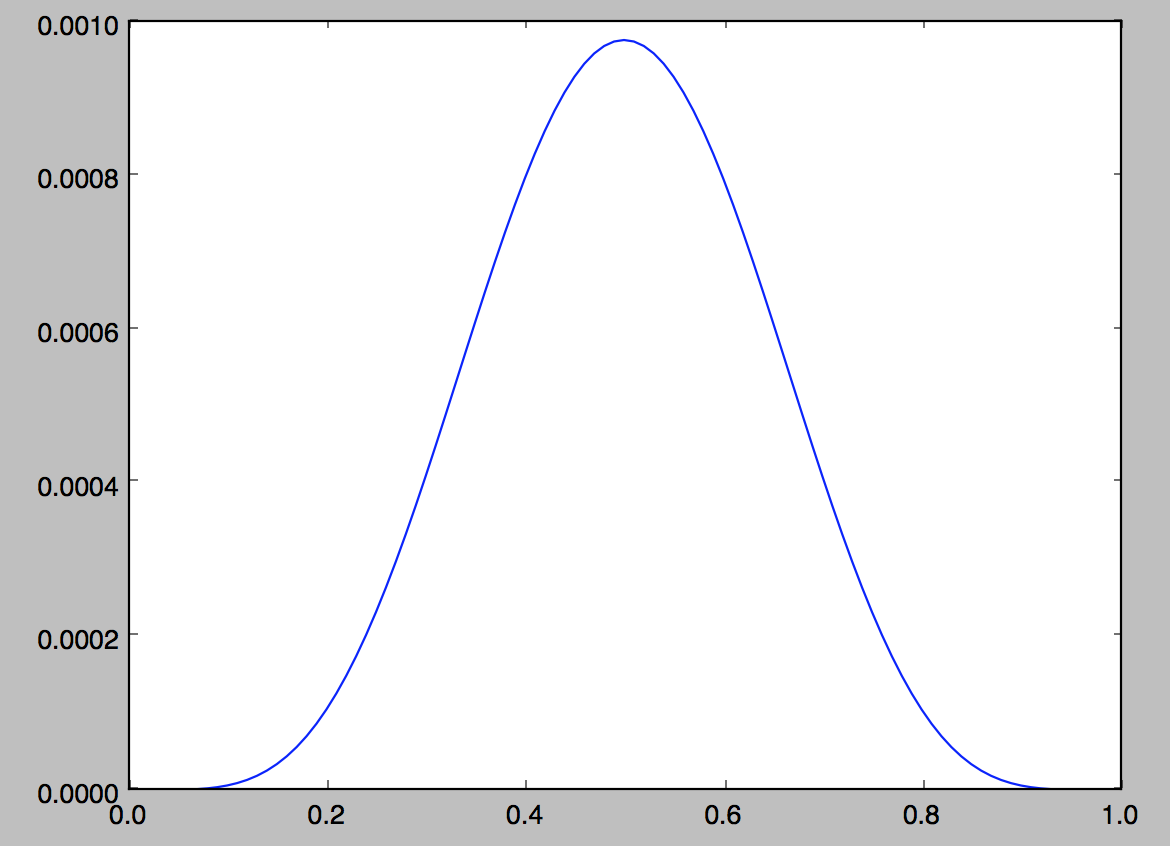
\includegraphics[scale=0.5]{five.png} \newline{}
For both the n = 5 and n = 100 datasets, the theta that maximized the likelihoods were both 0.6 (computer gave 0.5999999...). However, the maximum likelihoods themselves were 0.03456 and $5.9 * 10^{-30}$. This makes sense since it is much less likely to see a specific dataset from the bernoulli distribution if the dataset is very large, but since both datasets have the same expected value for X, the theta should be the same. For the n = 10 and 5 ones dataset, theta = 0.5 and ML = $9.7 * 10^{-4}$ was obtained. The parameter given by the plot matches the closed form answer, since for this dataset, $\theta = \bar{X} = 0.5$ \newline{} In general, the MLE is equivalent to the proportion of observed ones, and as we take $ n \longrightarrow{} \infty $ the function's spread narrows and the peak becomes more apparent, but the value of the likelihood decreases.

}
\end{enumerate}

\newpage
\section{Problem 2}

\solution{Solution to problem 2}
\begin{enumerate}
\item Problem 2a

\solution{
The best one-leaf decision tree will always predict a 1. Since the label is 0 when all the first three features are 0, we must compute the number of different arrangements such that the first three features are 0. This is $ 1 * 1 * 1 * 2 * 2 * ... 2 = 2^{n-3} $ possibilities. So the best decision tree will make $ 2^{n-3} $ mistakes, or an error rate of $ \frac{1}{8} $.
}

\vspace{1cm}
\item Problem 2b

\solution{
There is no such split. If we split on the value of $ X_i, i >=4$, the proportion of ones in each split will be the same ($\frac{7}{8}$) so a 1 will be predicted in both leaves. If we split on one of $X_i, i < 4 $, one leaf will have data that is only ones, and the proportion of data in the other leaf with label 1 will be $ \frac{7}{8} - \frac{1}{8} = \frac{3}{4} $. Therefore, the tree will predict 1 in both leaves. So any case with one split will make the same number of mistakes as a 1-leaf tree. 
}
\vspace{1cm}
\item Problem 2c
\solution{
\[ H[Y] = - \sum_{i = 1}^{K} P(X = a_i) log P(X = a_i) = \frac{1}{8}log(\frac{1}{8}) + \frac{7}{8}log(\frac{7}{8}) \] = 0.543
}

\vspace{1cm}
\item Problem 2d
\solution{
Yes. Using any of $ X_i, i <= 3 $ gives an entropy of $ \frac{1}{8}log(4) + \frac{3}{4}log(\frac{4}{3}) = 0.406 $
}
\end{enumerate}
\newpage
\section{Problem 3}
\solution{Solution to Problem 3}
\begin{enumerate}
\item Problem 3a
\solution{If $\frac{p_k}{p_k + n_k}$ is the same for all k, then we must have, for all k: \[\frac{p_k}{p_k + n_k} = \frac{p}{p + n} \]. Using the equation for gain, we obtain: \[G = B(\frac{p}{p + n}) - B(\frac{p}{p + n})\frac{1}{p + n} \sum_{k = 1}^{d} p_k + n_k \]
\[ = B(\frac{p}{p + n}) - B(\frac{p}{p + n})\frac{1}{p + n}(n + p) \]
\[ = B(\frac{p}{p + n}) - B(\frac{p}{p + n}) = 0 \]


}
\end{enumerate}
\newpage
\section{Problem 4}
\solution{Solution to Problem 4}
\begin{enumerate}
\item Problem 4a
\solution{ \newline{}
Pclass: Roughly the same number of people survived or didn't survive for a pclass value of 2. For first-class, about 60 more people survived than didn't. For pclass = 3, the didn't survive (survived = 0) was significantly higher. 
\newline{}
Sex: If sex = 0, survived was more frequent. For a value of 1, didn't survive was much more frequent. 
\newline{}
Age: The highest non-survival frequency age range was between 20 and 30 years. The only time the survived frequency is more than the didn't survive frequency is for ages between 0 and 10. 
\newline{}
SibSp: The sibSp value of 0 was the most common, and this value had a higher non-survival rate. For a SibSp value of 1, the rates are roughly equal with a few more surviving than not, and SipSp values of 3, 4, and 5 are relatively uncommon. 
\newline{}
Parch: The most frequent value was 0, for which a majority did not survive. For parch values of 1 and 2, the frequency of survival was slightly higher. A parch value of 3 through 7 was very uncommon. 
\newline{}
Fare: Those who paid the lowest fare had the highest non-survival ratio. As fare increased, the frequency of survival exceeds the frequency of non-survival. 
\newline{}
Embarked: The most frequent value was 2, which had a higher non-survival frequency. An embarked value of 0 had a higher survival rate, while the uncommon value of 1 had a slightly higher non-survival rate. 
}
\item Problem 4b
\solution{
I obtained a training error of 0.485.
}
\item Problem 4c
\solution{
The training error for sci-kit learn's DecisionTreeClassifier was 0.014. The "entropy" criterion was used, and all other parameters were unmodified.
}
\item Problem 4d
\solution{
The training and testing error were accumulated over n = 100 trials with an 80/20 random split of data. The errors were:
\newline{}
For DecisionTreeClassifier:
training error: 0.01230228471 \newline{}
test error: 0.243706293706
\newline{}
For RandomClassifier:
training error: 0.516695957821 \newline{}
test error: 0.482517482517

\newline{}
For MajorityClassifier: 
training error: 0.397188049209 \newline{}
test error: 0.433566433566
}
\item Problem 4e
\solution{
Plot of depths (1-20) vs training error: 
\newline{}
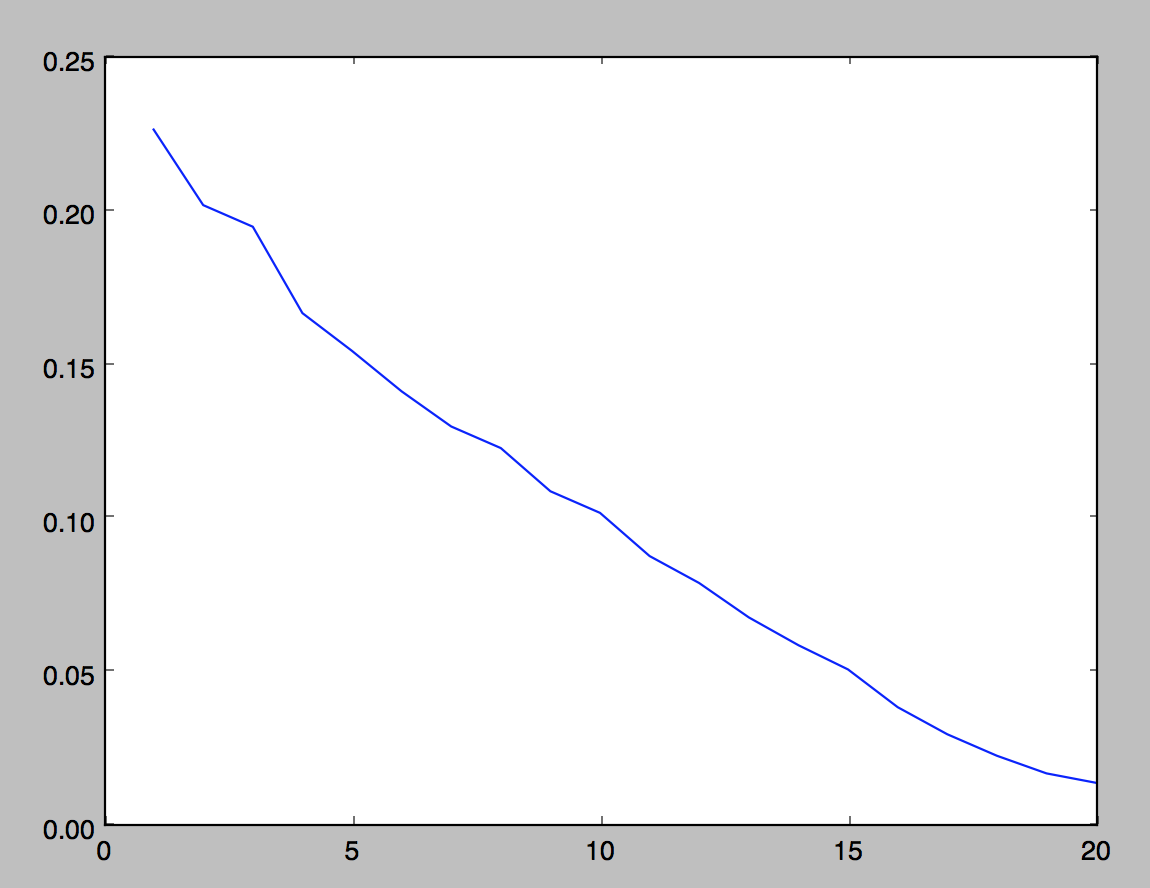
\includegraphics[scale=0.5]{training_error.png}
\newline{}
Plot of depths (1-20) vs testing error: 
\newline{}
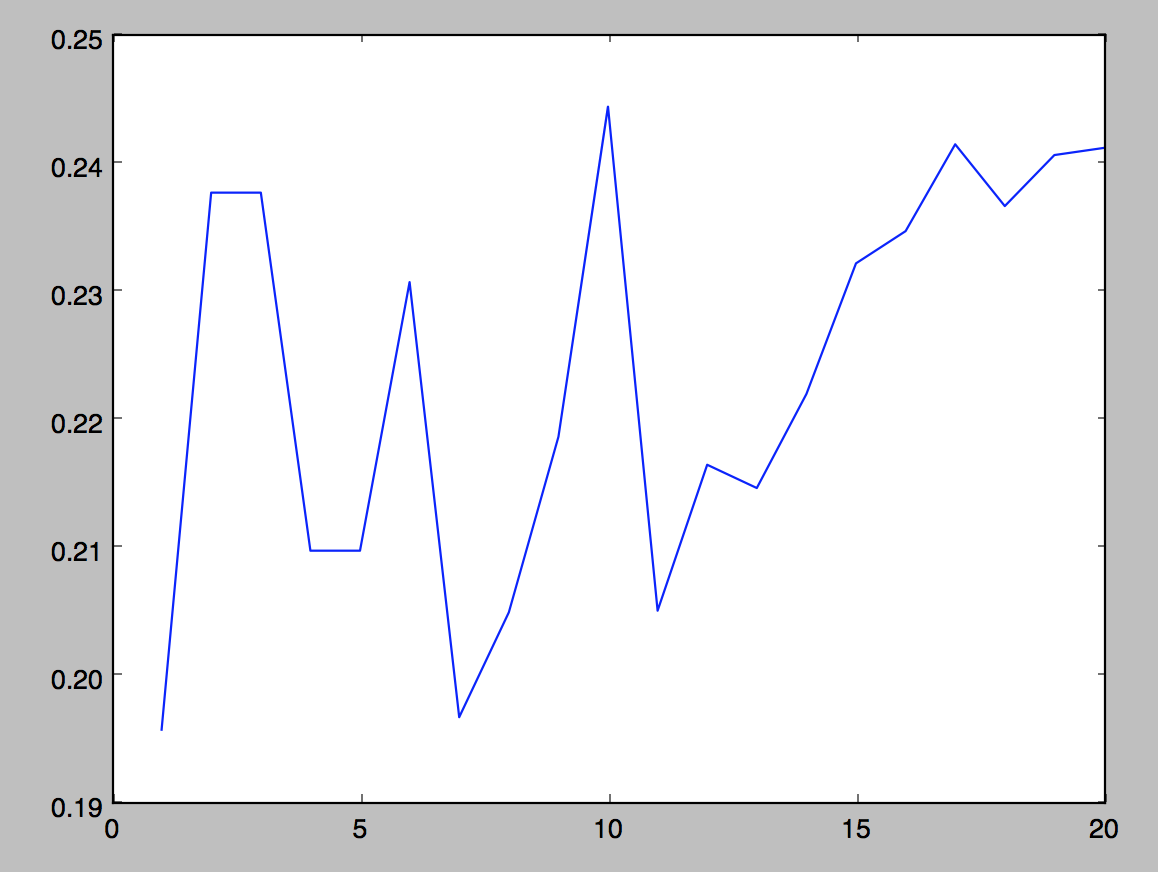
\includegraphics[scale=0.5]{testing_error.png}
\newline{}
We see overfitting as the maximum depth approaches 20. This is indicated by the continued reduction in error on the training data, but increased error on the testing data as our max depth increases. This indicates that the model has low bias and high variance, and has begun to "memorize" the training data. The best depth limit, if we consider the ability to generalize, should be determined by the error on the testing data. In this case, a max depth of 1 would minimize the training error the most, but a max depth of 7 is also a close second. 
}
\item Problem 4f
\solution{
\newline{}
Plot of splits against training error: 
\newline{}
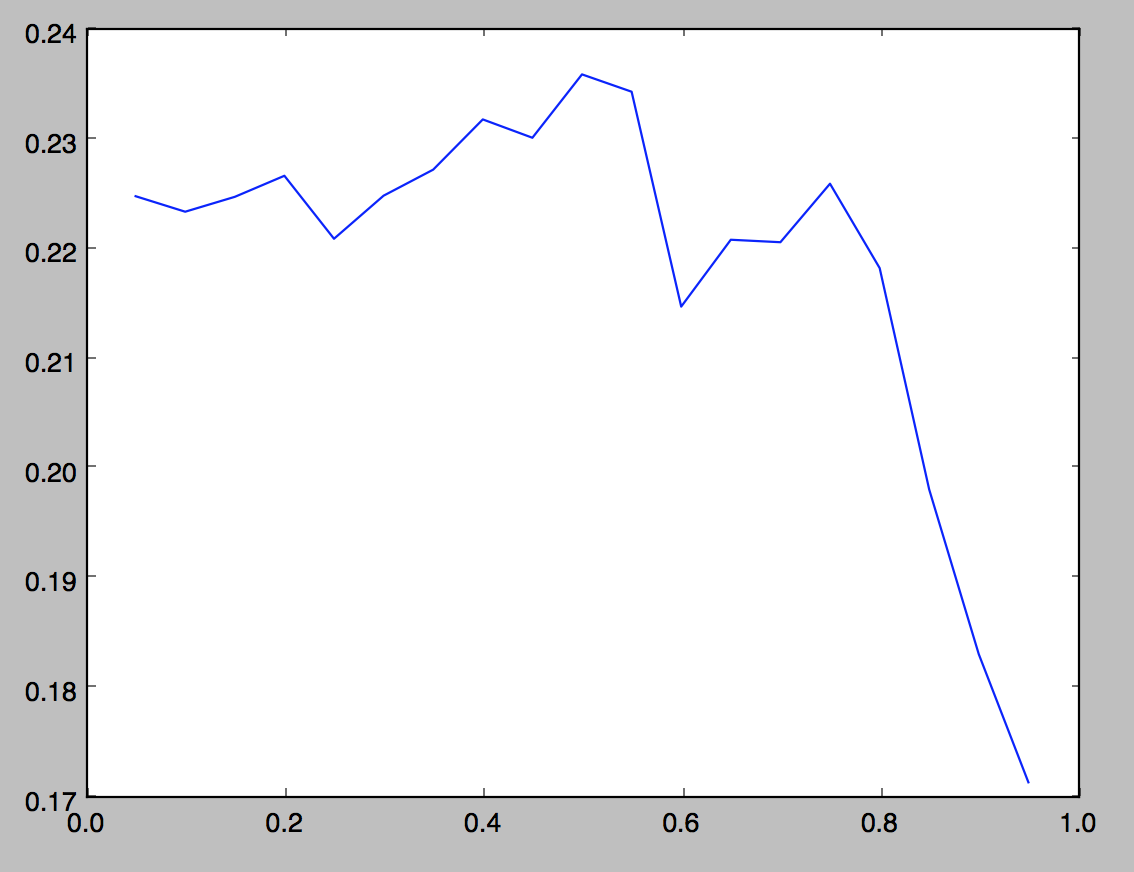
\includegraphics[scale=0.5]{data_training.png}
\newline{}
Plot of splits against testing error: 
\newline{}
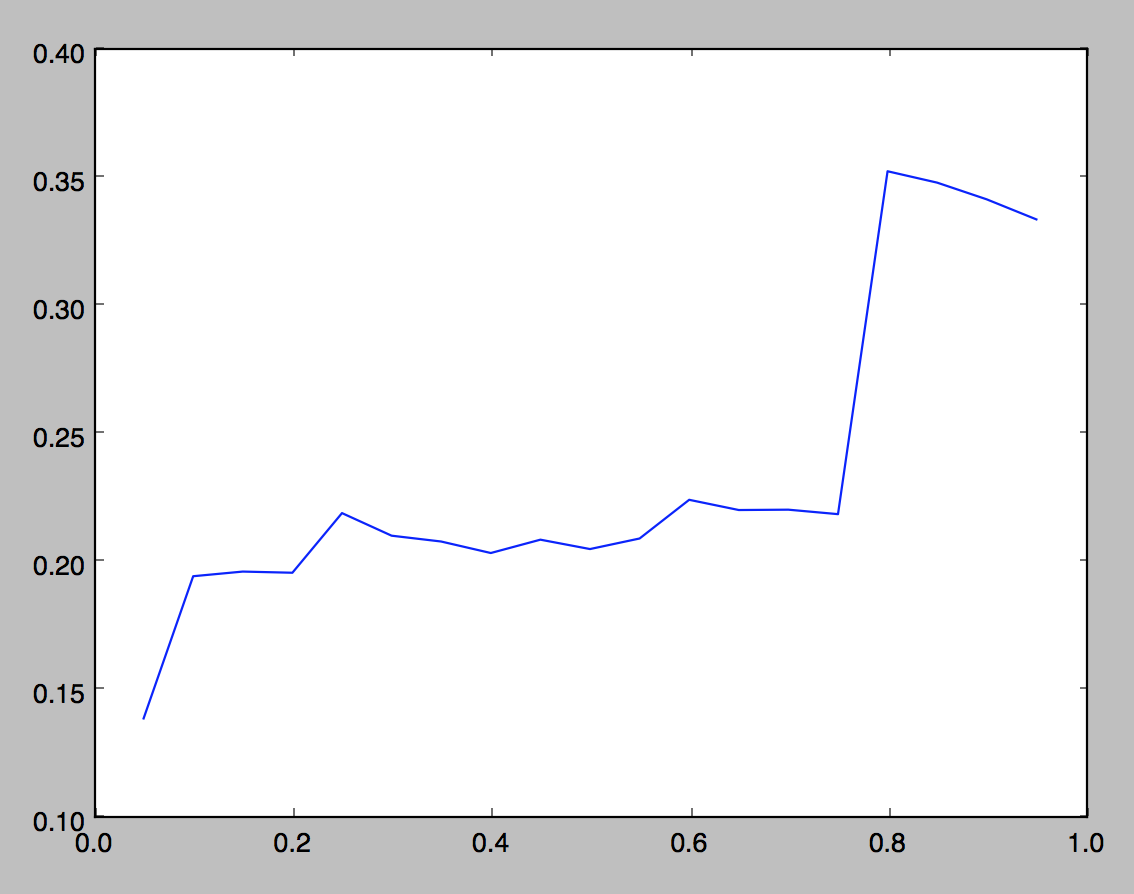
\includegraphics[scale=0.5]{data_test.png}
\newline{}
Similar to above, we again see overfitting as we use more data for training. This is again because we have more data to train on, so our classifier mistakes this data as more and more resemblent of the entire population, leading to worse generalization. 
}
\end{enumerate}
\end{document}
